\documentclass[onecolumn]{emulateapj}
%\documentclass[twocolumns]{emulateapj}
%apj gives the referee version/preprint2
%\usepackage[T1]{fontenc}
%\usepackage[utf8]{inputenc}
%\usepackage{graphicx}
%\usepackage{natbib}
\usepackage{amsmath}
\usepackage{amssymb}
%\usepackage{vmargin}
%\usepackage{pdfpages}
\usepackage{aas_macros}


\usepackage[normalem]{ulem}
\usepackage[usenames]{color}

\definecolor{DarkGreen}{rgb}{0.64,0.80,0.35}
\newcommand\ALc[1]{{\color{red} \bf #1}} %Astrid
\newcommand\Ac[1]{{\color{green} \bf #1}} %% Avery
\newcommand\Pc[1]{{\color{cyan} \bf #1}} %% Phil
\newcommand\Cc[1]{{\color{blue} \bf #1}} %% Christoph
\newcommand\Ec[1]{{\color{magenta} \bf #1}} %% Ewald

\begin{document}
\title{Blazar heating window function}

\author{A. Lamberts and P. Chang}
\affil{}
\email{lambera@uwm.edu}

%\altaffiltex{1}{Physics Department, UWM, Milwaukee WI 53211}

%\begin{abstract}
%Write a nice abstract here!


%\end{abstract}

%\keywords{BL Lacertae objects: general, cosmology: theory, gamma-rays: genereal, intergalactic medium, large-scale structure of universe}
%\section{Introduction}


\section {Determining the window function}\label{window}
The heating rate $\dot{q}$ can expressed as a mean heating rate $\bar{\dot{q}}$ plus a small fluctuation $\delta_H$.
\begin{equation}
  \label{eq:delta_h}
  \dot{q}=\bar{\dot{q}}(1+\delta_H).
\end{equation}

We map the heating fluctuations $\delta_H$ to the underlying dark matter overdensity in a given region $\delta$, by using a method that closely follows the work of  \citet{2007MNRAS.376.1680P} and \citet{2005ApJ...626....1B}. The overdensity of a region of radius $r$, centered on $\mathbf{x}$ is given by
\begin{equation}
  \label{eq:delta}
  \delta(\mathbf{x},r)=\frac{\rho(\mathbf{x})-\bar{\rho}(r)}{\bar{\rho}(r)}
\end{equation}
with $\rho$ the local density and $\bar{\rho}$ its average over the whole region. The method is based on a Taylor expansion of the quantities describing the TeV sources and keeping only the first order corrections in Fourier space.  We thus have
\begin{equation}
  \label{eq:use_window}
  \tilde{\delta}_H=W_H\tilde{\delta},
\end{equation}
where $W_H$ is defined as the window function and maps the Fourier transform of the overdensity, $\tilde{\delta}$, to the Fourier transform of the heating fluctuations, $\tilde{\delta}_H$ . This naturally yields the significant lengthscale for heating fluctuations. 
The detaild exposition of this method, in the Newtonian limit and in an expanding universe, is given in Appendix A. In the following section, we present the general method and highlight the underlying hypotheses of our work.

\subsection{Window function for TeV blazar heating}
The heating rate at a given point $\mathbf{x}$ is determined by the received TeV flux from all the sources within a certain radius $r_{max}$, where $r_{max} \gg $ the mean free path of VHEGRs. We assume that the TeV photons that are converted to pairs via interaction with the EBL lose their energy to the IGM at the point where they are created.  As stated in \citet{2012ApJ...752...22B}, this is a reasonable assumption as the plasma instability lengthscales are significantly smaller than the mean free path of these TeV photons. The heating rate per baryon at a given point is 
\begin{equation}
\label{eq:heating_rate}
  \dot{q}(\mathbf{x})= \frac{E_0}{4\pi}  \int_{\Omega}\int_0^{r_{max}}   \mathcal{E}(\mathbf{r}'+\mathbf{x})\sigma  e^{-\tau}d\Omega dr' ,
\end{equation}

 $E_0$ is the mean energy of the TeV photons and   $\mathcal{E}$ is the emissivity of the sources (photons per unit time, per unit volume). $\sigma$ (in cm$^{-2}$) is the energy-averaged cross section for pair production on the extragalactic background light and $\tau$ is the associated optical depth along the line of sight. 
\begin{equation}
\label{eq:heating_rate}
  \dot{q}(\mathbf{x})= \frac{1} {4\pi}  \int_{\Omega}\int_0^{r_{max}}   \mathcal{E}(\mathbf{r}'+\mathbf{x})\sigma  e^{-\tau(\mathbf{r}')}d\Omega dr' ,
\end{equation}
$\mathcal{E}$ is the emissivity of the sources (photons per unit time, per unit volume). $\sigma$ (in cm$^{-2}$) is the energy-averaged cross section for pair production on the extragalactic background light and $\tau$ is the associated optical depth along the line of sight. 

 
 
One can then express the emissivity as a mean value and a first order correction. The TeV emissivity is related to the presence of a supermassive black holes at centers of galaxies, which cluster in overdense regions. On average, larger overdensities contain larger number of galaxies (reflected in their bias) and hence are more prominent sources of TeV emission.  Matter is tightly coupled to the underlying dark matter, which evolution is easy to model analytically within the linear approximation.  The linear approximation is valid as long as the overdensity is small, which is always true in the early universe and then breaks down at small scales as very dense structures form.  Our computation takes into account the bias between baryonic matter and dark matter \citep{1996MNRAS.282..347M}. To model cosmic distances, Eq.~\ref{eq:heating_rate} is integrated in redshift space and we take into account the resulting energy loss for the TeV photons as well as the first order corrections due to proper motions of the sources within the Hubble flow \citep{1987MNRAS.227....1K}. We integrate over the energy distribution of the TeV-emission . 

% \begin{equation}
%   \label{eq:use_window}
%   \tilde{\delta}_H=W_H\tilde{\delta}.
% \end{equation}
\begin{eqnarray}
  \label{eq:window}
  \tilde{W}_H(k,z)&=&\frac{1}{\bar{X}}\int_{E_{min}}^{E_{max}}dE\int_z^{z_{max}}\frac{dX(E,z,z')}{dz'} \\ 
&&\times \frac{D(z')}{D(z)}\left((b(z)+1)j_0(kr)-\frac{2}{3}j_2(kr)\right)dz', \nonumber
\end{eqnarray}

with 
 \begin{equation}
  \label{eq:define_X}
  X(E,z',z)=\frac{e^{-\tau(z,z',E)}(1+z)^2}{H(z')\epsilon(E',z')}.
\end{equation}

%\Pc{where $W_H$ is defined as the window function and maps the Fourier transform of the overdensity, $\tilde{\delta}$, to the Fourier transform of the heating fluctuations, $\tilde{\delta}_H$ }
and $\bar{X}$ its spectral average. $E$ is the energy of the received TeV photon and, $E'$ its initial energy and  $\epsilon$ the blazar luminosity density. $b$ is the mass averaged bias and $j_0$ and $j_2$ spherical Bessel functions.


Assuming the TeV blazar distribution follows the redshift evolution of quasars, \citet{2012ApJ...752...22B} determined the blazar luminosity density in the TeV band based on a fit to \citet{2007ApJ...654..731H}

\begin{eqnarray}
  \label{eq:mean_heat}
  \mathcal{E}(E',z)&=&\mathcal{E}(E',z=0)\Phi_{B}(z)\\ \nonumber
&\simeq& \zeta\epsilon(E',z=0)\Phi_{Q}(z),
%&\simeq& \zeta\epsilon(E',z=0)10^{-.0037(1+z)^4+.085(1+z)^3-.0778(1+z)^2+2.795(1+z)-2.133}
\end{eqnarray}
with $\zeta=3.8\times 10^{-3}$ and
\begin{equation}
  \label{eq:phi_quasar}
 \Phi_{Q}(z)=10^{-.0037(1+z)^4+.085(1+z)^3-.0778(1+z)^2+2.795(1+z)-2.133}. 
\end{equation}
 

As the spectra of TeV blazars follow a power law with intrinsic (i.e. redshift corrected) spectral index $\alpha$ , one has

\begin{equation}
  \label{eq:blaz_lum}
  \epsilon(E',z=0)=\epsilon(E_0,z=0)\left(\frac{E'}{E_0}\right)^{-\alpha}\equiv \epsilon_0\left(\frac{E'}{E_0}\right)^{-\alpha},
\end{equation}
with $\epsilon_0=(1.7-4.8)\times 10^{-36}$erg s$^{-1}$ cm$^{-3}=(.5-1.4)\times 10^{38}$ erg s$^{-1}$ Mpc$^{-3}$ the current blazar luminosity density. Using 28 TeV blazars, \citet{2012ApJ...752...23C} find that $\alpha\simeq 3$ and $E_0\simeq $ 1 TeV. Following the emission of the nearest TeV blazars, we use $E_{min}=100$ GeV,  and $E_{max}=10$ TeV. Assuming blazars follow a similar evolution to quasars, we use $z_{maz}=5$  \citep{2007ApJ...654..731H}.

The optical depth is set by the mean free path  $D_{pp}(E',z)$ of  TeV photons before they interact with an EBL photon and produce and electron-positron pair. Its redshift evolution is set by the EBL and is hard to constrain as it is related to the star formation history of the universe as well as its metalicity and dust contents (see e.g \citet{2008A&A...487..837F,2006ApJ...648..774S}).  Following \citet{2012ApJ...752...23C} we use  a prescription 

  \begin{equation}
    \label{eq:mean_free_path}
  D_{pp}(E,z)=35\left(\frac{E}{1 \quad\textrm{TeV}}\right)^{-1} \left(\frac{1+z}{2}\right)^{-\xi} \quad \textrm{Mpc,}   
  \end{equation}

where $\xi=4.5$ for $z<1$ and $\xi=0$ for $z>1$ \citep{2004A&A...413..807K,2009PhRvD..80l3012N}. 

Using Eqs ~\ref{eq:mean_heat} and \ref{eq:mean_free_path} in Eq.~\ref{eq:window} then gives the complete window function for TeV blazar heating as shown of Fig. \ref{fig:window} for $z=0,2$ and 4. We have computed the window function using an embedded Runge-Kutta method which is able to capture the fast variation of the Bessel functions at large wavenumbers while decreasing computing time at smaller wavenumbers. To avoid unnecessary computations, we set both Bessel functions to zero when $kr$ is larger than 50. We checked this does not affect the final result.
%\textit{Discuss problems at low z, high k?}.

\begin{figure}[h]
  \centering
  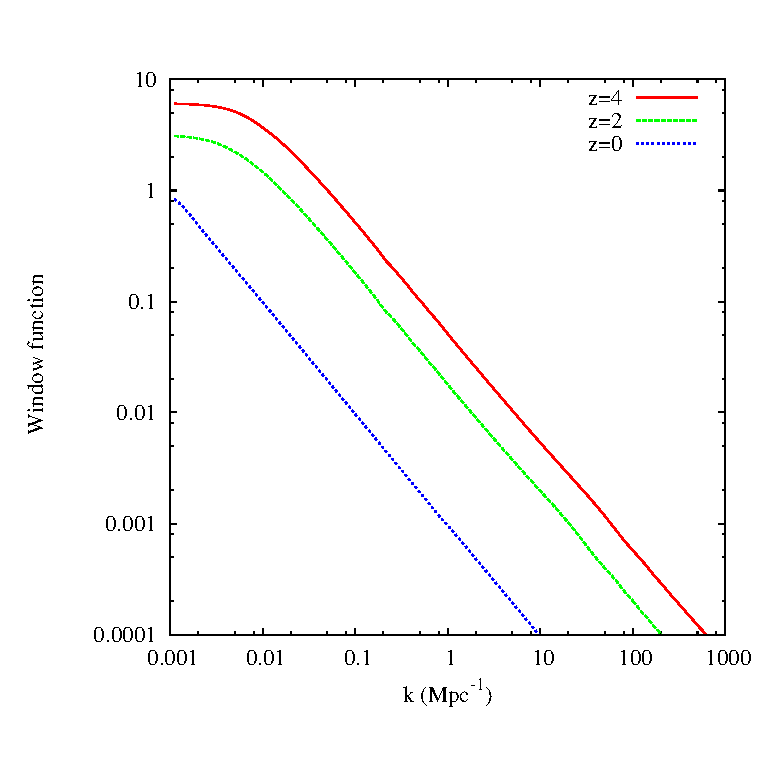
\includegraphics[width = .45\textwidth ]{full_window}
  \caption{Window function for TeV blazar heating from z=0 (blue dotted line), z=2 (green dashed line) and z=4 (full red line) .}
  \label{fig:window}
\end{figure}

% The window function describes how density fluctuations translate into heating fluctuations. Especially at low redshift, all the power resides in the large scales, meaning blazar heating is uniform regardless of the density distribution. At the current epoch,  the TeV blazar heating is uniform as the heating fluctuations trace density fluctuations at scales larger than 100 Mpc, where the Universe is essentially uniform  (see \citet{2013MNRAS.429.2910C} and references therein).  At lower redshift, overdensities at scales down to a few Mpc, or the size of typical clusters can impact the local heating rate. As the window function remains positive at all scales, underdense regions such as voids are the only areas where a lower than average heating rate is expected. Above average  heating is possible in large scale overdensities but also at  smaller scales when the overdensity is important. However, in such regions the linear theory for the dark matter evolution breaks down and we will not consider such cases. After these first anaytical estimates, we include the window function to model TeV blazar heating in cosmological simulations.


 \section{Details (appendix of the paper)}
We detail the derivation of the window function in Eq. \ref{eq:window}. We start from a purely Newtonian universe, then include the impact of expansion and finally the various first order corrections to the received TeV flux.
\subsection {Newtonian case}\label{sec:windon_newt}

\subsubsection {Fluctuations with respect to the mean heating rate}

The TeV flux received (in photons s$^{-1}$ cm$^{-2}$) at position $\mathbf{x}$ is given by the sum over all the sources within a radius $r\leqslant r_{max}$.
\begin{equation}
  \label{eq:flux_recu0}
  J(\mathbf{x})=\int_{0}^{2\pi}\int_{0}^{\pi}\int_0^{r_{max}}   \frac{\mathcal{E}(\mathbf{x}') }{4\pi |\mathbf{x}'-\mathbf{x}|^2} e^{-\tau} |\mathbf{x}'-\mathbf{x}|^2 \sin\theta d\theta d\phi d(\mathbf{x}'-\mathbf{x}),
\end{equation}
where the emissivity $\mathcal{E}$ is given in photons per unit time, per unit volume. $\tau=\kappa (\mathbf{x}'-\mathbf{x})$ is the optical depth along the line of sight, $\kappa$ the absorption coefficient.
Introducing $\mathbf{r'}=\mathbf{x}'-\mathbf{x}$, and $d\Omega=sin\theta d\theta d\phi$ this gives


\begin{equation}
  \label{eq:flux_recu}
  J(\mathbf{x})=\int_{\Omega}\int_0^{r_{max}}   \frac{\mathcal{E}(\mathbf{r}'+\mathbf{x}) }{4\pi } e^{-\tau} d\Omega dr'.
\end{equation}

The corresponding heating rate (erg cm$^{-3}$ s$^{-1}$ ) is given by 
\begin{equation}
  \label{eq:heating_rate0}
  \dot{Q}(\mathbf{x})=\frac{E_0}{D_{pp}}J(\mathbf{x}) =\frac{E}{4\pi}   \int_{\Omega}d\Omega\int_0^{r_{max}}   \mathcal{E}(\mathbf{r}'+\mathbf{x}) \frac{1}{D_{pp}}  e^{-\tau} dr' ,
\end{equation}
with $E_0$ the mean energy of the TeV photons and $D_{pp}$ their mean free path  before they pair-produce. For convenience reasons,  we will not take into account the impact of the spectral energy distribution of the TeV photons in this Appendix. It is taken into account in the exact computation in section \S\ref{window}.

This gives the  heating rate per baryon
\begin{equation}
  \label{eq:heating_rate0}
  \dot{q}(\mathbf{x})=\frac{\dot{Q}}{n}= \frac{E_0}{4\pi}  \int_{\Omega}\int_0^{r_{max}}   \mathcal{E}(\mathbf{r}'+\mathbf{x})\sigma  e^{-\tau}d\Omega dr' ,
\end{equation}
where $n$ is the average density of the target photons (i.e. the EBL) and $\sigma$ (in cm$^{-2}$) is the energy averaged cross section for pair production on the extragalactic background light (EBL) photons \citep{1967PhRv..155.1408G}. 


The mean heating rate can be expressed as
\begin{equation}
  \label{eq:heating_rate0}
  \bar{\dot{q}}=\frac{E_0}{4\pi} \int_{\Omega}d\Omega\int_0^{r_{max}}  \bar{\mathcal{E}}\sigma  e^{-\tau}dr', 
\end{equation}
with $\bar{\mathcal{E}}$ the mean emissivity. Throughout the whole appendix, barred quantities are spatially averaged quantities.

The heating rate fluctuations at a given point are then given by 

\begin{eqnarray}
  \label{eq:heat_fluc_newt0}
  \delta_H(\mathbf{x})&=&\frac{\dot{q}(\mathbf{x})-\bar{\dot{q}}}{\bar{\dot{q}}}=\frac{E_0}{4\pi\bar{\dot{q}}} \int_{\Omega}d\Omega\int_0^{r_{max}}   (\mathcal{E}(\mathbf{r}'+\mathbf{x})-\bar{\mathcal{E}}) \sigma  e^{-\tau} dr' \\ \nonumber
  &=&\frac{E_0}{4\pi\bar{\dot{q}}}\int_{\Omega}d\Omega\int_0^{r_{max}}   \delta_E(\mathbf{r}'+\mathbf{x})\bar{\mathcal{E}}\sigma  e^{-\kappa r'}dr',
\end{eqnarray}
with the fluctuations in the TeV emissivity.
\begin{equation}
  \label{eq:fluc_emissivity}
  \delta_E(\mathbf{r}'+\mathbf{x})=\frac{\mathcal{E}(\mathbf{r'}+\mathbf{x})-\bar{\mathcal{E}}}{\bar{\mathcal{E}}}.
\end{equation}

If  the emissivity is directly related to the density, one has $\delta_E=\delta$.

\subsubsection{Window function}
As the universe is infinite and asymptotically flat, we can expand the fluctuations into planar waves, in order to get the lengthscale dependence of heating rate fluctuations \citep{2004MNRAS.352..142B}.

\begin{eqnarray}
  \label{eq:FT_delta}
  \delta_H(\mathbf{x})&=&\frac{1}{(2\pi)^3}\int_{-\infty}^{\infty} d^3\mathbf{k'} \tilde{\delta}_H(\mathbf{k'}) e^{-i\mathbf{k'}\cdot\mathbf{x}}\\ \nonumber
  \delta_E(\mathbf{r}'+\mathbf{x})&=&\frac{1}{(2\pi)^3}\int d^3\mathbf{k'} \tilde{\delta}_E(\mathbf{k'}) e^{-i\mathbf{k'}\cdot(\mathbf{r'}+\mathbf{x})},
\end{eqnarray}
where the $\tilde{}$ indicates a Fourier transform.
This gives
\begin{eqnarray}
  \label{eq:heat_fluc_newt1}
\frac{E_0}{(2\pi)^3}\int_{-\infty}^{\infty} d^3\mathbf{k'} \tilde{\delta}_H(\mathbf{k'}) e^{-i\mathbf{k'}\cdot\mathbf{x}}&=&\frac{1}{4\pi\bar{\dot{q}}_0} \int_{\Omega}d\Omega\int_0^{r_{max}}   \bar{\mathcal{E}}\sigma  e^{-\kappa r'}  \frac{1}{(2\pi)^3}\int d^3\mathbf{k'} \tilde{\delta}_E(\mathbf{k'}) e^{-i\mathbf{k'}\cdot(\mathbf{r'}+\mathbf{x})} dr'.
\end{eqnarray}

% To illustrate the next step, we perform a Fourier transform on Eq.\ref{eq:FFT} 
% \begin{eqnarray}
%   \label{eq:left}
% \frac{\tilde(\delta)(k)}{(2\pi)^3}&=&\frac{1}{(2\pi)^3}\int d^3\mathbf{k'}\tilde{\delta}(\mathbf{k'}) \int d^3\mathbf{x} e^{i(\mathbf{k}-\mathbf{k}')\cdot \mathbf{x}} \\
%  &=&  \frac{1}{(2\pi)^3}\int d^3\mathbf{k}'\delta^{(0)}(\mathbf{k}-\mathbf{k}')\tilde{\delta}_H(\mathbf{k}')\\
%   &=&  \frac{1}{(2\pi)^3} \tilde{\delta}_H(\mathbf{k})
% \end{eqnarray}




Performing a Fourier transform on the right-hand side of Eq.\ref{eq:heat_fluc_newt0}, we have
\begin{eqnarray}
  \label{eq:right}
  &=& \frac{1}{(2\pi)^3} \frac{E_0}{4\pi\bar{\dot{q}}}\int_{\Omega}d\Omega\int_0^{r_{max}} \bar{ \mathcal{E}}\sigma  e^{-\kappa r'} \int d^3\mathbf{k'}\int d^3\mathbf{x} \tilde{\delta}_E(\mathbf{k'})e^{-i\mathbf{k'}\cdot{\mathbf{r}'}} e^{i(\mathbf{k}-\mathbf{k'})\cdot\mathbf{x}}  dr'\\ \nonumber
  &=&\frac{1}{(2\pi)^3} \frac{E_0}{4\pi\bar{\dot{q}}} \int_{\Omega}d\Omega\int_0^{r_{max}}   \bar{\mathcal{E}}\sigma  e^{-\kappa r'} \int d^3\mathbf{k'} \delta^{0}(\mathbf{k}-\mathbf{k}')e^{-i\mathbf{k'}\cdot{\mathbf{r}'}} \tilde{\delta}_E(\mathbf{k'})    dr'\\ \nonumber
  &=&\frac{1}{(2\pi)^3} \frac{E_0}{4\pi\bar{\dot{q}}} \int_{\Omega}d\Omega\int_0^{r_{max}}  \bar{ \mathcal{E}}\sigma  e^{-\kappa r'}  \tilde{\delta}_E(\mathbf{k}) e^{-i\mathbf{k}\cdot{\mathbf{r}'}}  dr',
\end{eqnarray}
with $\delta^{(0)}$ the Dirac function, which Fourier transform equals 1. Introducing $\mu=cos\theta$, where $\theta$ is the angle between the wavevector and the line of sight, Eq. \ref{eq:heat_fluc_newt0} rewrites
\begin{eqnarray}
  \label{eq:heat_fluc_newt1}
  \tilde{\delta}_H(\mathbf{k})&=&  \frac{E_0}{\bar{2\dot{q}}} \int_{-1}^{1} d\mu \int_0^{r_{max}}  \bar{\mathcal{E}}\sigma  e^{-\kappa r'}  \tilde{\delta}_E(k) e^{-ikr'\mu}  dr'\\ \nonumber
&=&\tilde{\delta}_E(\mathbf{k})\frac{\sigma E_0}{\bar{\dot{q}}}\int_0^{r_{max}} \frac{sin(kr')}{kr'}   \bar{\mathcal{E}}  e^{-\kappa r'}   dr'.\\ \nonumber
%&=&\tilde{\delta}_E(\mathbf{k})\frac{\sigma E_0}{ \bar{\dot{q}}\kappa}  \frac{atan(k)}{k}\\ \nonumber
%&=&\tilde{\delta}_E(\mathbf{k}) \frac{atan(k)}{k}.
\end{eqnarray}

Fig.\ref{fig:window_newt} shows  window functions with different absorption coefficients in a purely Newtonian universe. The solid red line shows a case with no absorption, the dashed green line shows a case with $\kappa=10$ Mpc$^{-1}$.  In the former case, large scale sctructure has the strongest impact on heating, as larger regions have more sources. When absorption is present,  the impact of large scale structure (i.e. low k) remains constant as distant sources are absorbed. In such case, for scales equal to or larger than the cutoff, heating fluctuations follow density fluctuations and overdense regions get more heat. At smaller scales, the density structure has less impact on the heating, unless a strong overdensity is present.  

\begin{figure}
  \centering
  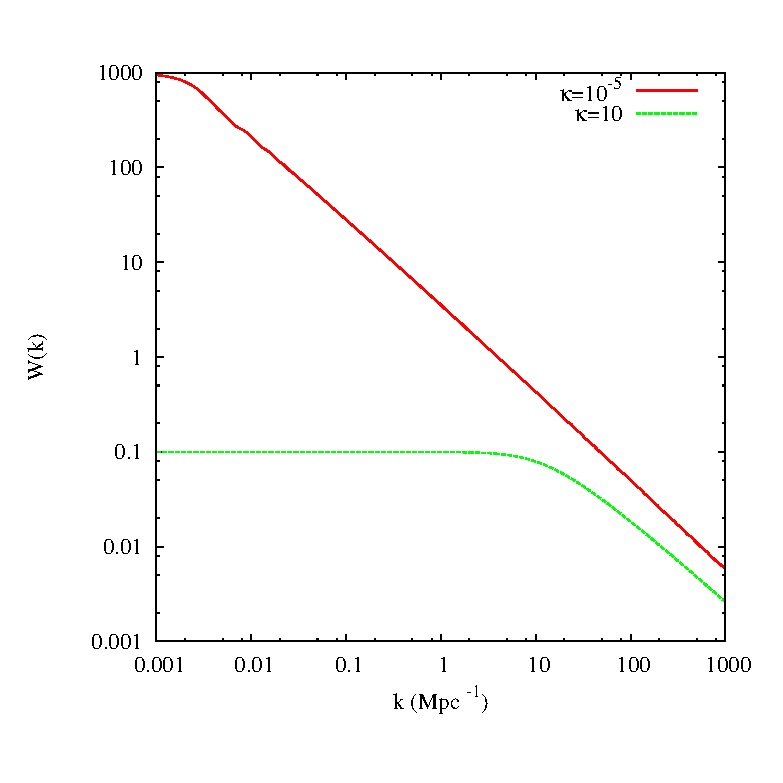
\includegraphics[width = .45\textwidth ]{newtonian_window}
  \caption{Window function for a non-expanding universe. The solid red line has very little absorption ($\kappa=10^{-5}$ Mpc$^{-1}$), the dashed green line has $\kappa=10 $ Mpc$^{-1}$ .}
  \label{fig:window_newt}
\end{figure}



\subsection{Expanding universe}\label{sec:window_exp}

We perform the same derivation as in the former section, replacing the integrals on the (proper) distance by redshift integrals using
\begin{equation}
  \label{eq:proper_dist}
  dr=\int \frac{c}{H(z)(1+z')} dz'.
\end{equation}
where  $H(z)$ is the Hubble parameter.

 The emissivity $\mathcal{E}$ is given in comoving units, while the heating rate  is expressed in proper units. The proper volume is  $(1+z)^3$ times larger than the comoving volume. 
Let $\mathbf{s}$ a point with coordinates $(z,\theta,\phi)$, the heating rate at $\mathbf{s}$ is 

\begin{equation}
  \label{eq:int_exp_heat}
  \dot{q}(\mathbf{s})=\frac{E_0(1+z)^2}{4\pi}\int_{\Omega}d\Omega\int_z^{z_{max}}\frac{dl}{dz'}\sigma\mathcal{E}(E',z') e^{-\tau} dz'.
\end{equation}
 $z'=z+\Delta z$, with $\Delta z$ the difference in redshift between the emission and reception of the photons.

$\mathcal{E}(E',z')$ is  the   blazar luminosity at the energy $E'$,  which then redshifts to energy $E$ following 
\begin{equation}
  \label{eq:E_z}
  E'=E\frac{1+z}{1+z'}.
\end{equation}

$\tau(E,z',z)$ is the optical depth of a TeV photon observed at redshift $z$ with energy $E$, which was emitted at redshift $z'$ with energy $E'$.

\begin{equation}
  \label{eq:tau}
  \tau(E,z',z)=\int_z^{z'}dz''\frac{1}{D_{pp}}\frac{dl}{dz''}=\int_z^{z'}dz''\frac{c}{H(z'')(1+z'')}\frac{1}{D_{pp}},
\end{equation}



The mean heating rate is given by 
\begin{equation}
  \label{eq:mean_exp_heat}
  \bar{\dot{q}}=\frac{E_0(1+z)^2}{4\pi}\int_{\Omega}d\Omega\int \frac{dl}{dz'}\sigma\bar{\mathcal{E}} e^{-\tau}dz'.
\end{equation}
%\textit{Here I'm not quite sure about the boundaries for the integral. Should we integrate from z=0 to zmax? I'm also puzzled about what to do with the redshift of the energy.}

The resulting heating rate fluctuations are then given by

\begin{eqnarray}
  \label{eq:fluc_exp0}
  \delta_H(\mathbf{s})&=&\frac{\dot{q}(\mathbf{s})-\bar{\dot{q}}}{\bar{\dot{q}}}=\frac{E_0(1+z)^2c\sigma}{4\pi\bar{\dot{q}}} \int_{\Omega}d\Omega\int_z^{z_{max}} \frac{ ( \mathcal{E}(z')-\bar{\mathcal{E}})  e^{-\tau}}{H(z')} dz' \\ \nonumber
  &=&\frac{E_0(1+z)^2\bar{\mathcal{E}} c\sigma}{4\pi\bar{\dot{q}}}  \int_{\Omega}d\Omega\int_0^{z_{max}}   \frac{\delta_E(z')  e^{-\tau}}{H(z')}dz'.
\end{eqnarray}

The TeV emission is related to the presence of supermassive black holes at the center of galaxies, which are located in collapsed dark matter halos.  We can thus connect the fluctuations of the TeV emission, within a certain radius $r$, to the underlying dark matter fluctuations $\delta$, defined by Eq. \ref{eq:delta}.
% \begin{equation}
%   \label{eq:delta}
%   \delta(z,r)=\frac{\rho(z,r)-\bar{\rho}(z)}{\bar{\rho}(z)},
% \end{equation}

% where $\rho$ is the dark matter  density of the Universe. 

At this stage we assume the TeV fluctuations exactly match the dark matter fluctuations $\delta_E=\delta$.  We will see in the next section that this is not exactly true and will take into account various corrections.  The initial density fluctuations represent a Gaussian random field, which exact properties depend on the earliest stages of the Universe prior to recombination \citep{1986ApJ...304...15B,Peebles}. Then they grow linearly between $z'$ and $z$ following $\delta(z',r)=\delta_0(r)D(z')/D(z)$ \citep{ 1977MNRAS.179..351H}.

\begin{equation}
  \label{eq:growth_1}
  D(z)=D_0H(z)\int_z^{\infty}\frac{1+z'}{H^3(z')}dz'.
\end{equation}
%The dark matter fluctuations initially grow linearly as the different Fourier modes of $\delta(\mathbf{k})$ evolve at the same rate, independently. 
The linear approximation breaks down when the amplitude of the root mean square of the perturbations approaches unity. The evolution of the density field is then determined by the spherical collapse \citep{1972ApJ...176....1G} and the virialization of halos. As the growth of the modes is independent of the wavenumber, we have

\begin{equation}
  \label{eq:FT_delta}
  \delta_E(z',r)=\delta(z',r)=\delta_o(r)D(z')=\delta_0D(z')\frac{1}{(2\pi)^3}\int d^3\mathbf{k'} \tilde{\delta}(\mathbf{k'}) e^{-i\mathbf{k'}\cdot\mathbf{r}}.
\end{equation}


And Eq. \ref{eq:fluc_exp0}  rewrites as
\begin{equation}
  \label{eq:heat_fluc_exp0}
  \delta_H(\mathbf{s})=\frac{c\sigma\bar{\mathcal{E}} E_0(1+z)^2 }{4\pi\bar{\dot{q}}} \int_{\Omega}d\Omega\int_z^{z_{max}}  \frac{D(z')}{D(z)} \frac{\delta(r') e^{-\tau}}{H(z')}dz'.
\end{equation}


The left hand side yields $\tilde{\delta}(\mathbf{k})$ while the right hand side transforms in a similar fashion to Eq. \ref{eq:right}. As the power spectrum of density fluctuations is isotropic, this  yields

\begin{equation}
  \label{eq:heat_fluc_exp1}
  \tilde{\delta}_H(k)=\tilde{\delta}(k) \frac{c \sigma \bar{\mathcal{E}}E_0(1+z)^2}{\bar{\dot{q}}} \int_z^{z_{max}} \frac{D(z')}{D(z)}\frac{sin(kr'(z'))}{kr'(z')}    \frac{e^{-\kappa r'(z')}} {H(z')}  dz'.
\end{equation}

%\begin{figure}[h]               
%  \centering
%  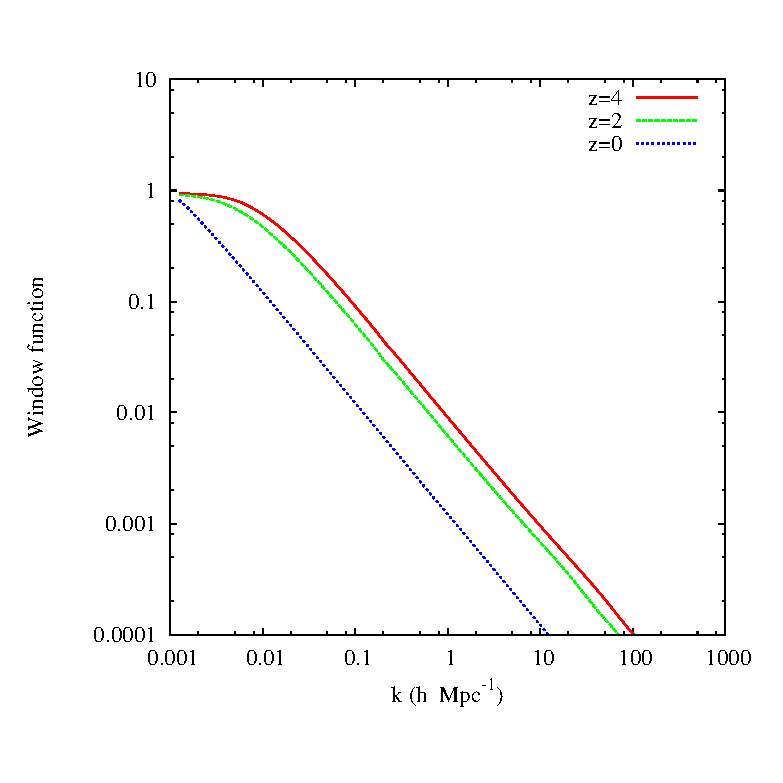
\includegraphics[width = .45\textwidth ]{window_nobiases}
%  \caption{Window function in an expanding universe.}
%  \label{fig:window_nobiases}
%\end{figure}

%Fig. \ref{fig:window_nobiases} shows the window function in an expanding universe.  Comparing with non-expanding case in Fig. \ref{fig:window_newt} \textit{ blabla} 
The TeV emission fluctuations are not exactly equal to the DM density fluctuations. In the next section we will account for the various corrections that have to be taken into account to determine a more accurate window function.


\subsection{Complete window function}

%
\subsubsection{Galaxy bias}
The TeV flux fluctuations are related to the distribution of galaxies, which is biased with respect to the distribution of dark matter halos, which in turn is biased with repect to the initial linear dark matter density fluctuations  \citep{1996MNRAS.282..347M}.  One defines the galaxy bias as the ratio between the power spectrum of galaxies to the power spectrum of the DM halos (see e.g. \citep{2002PhR...372....1C} for a review).  Galaxies bias is usually derived from simulations \citep{1999MNRAS.307..529K}, and observations for low redshifts \citep{2004ApJ...606..702T}. Galaxy bias is only weakly dependent on scale \citep{1998MNRAS.293..209M}, especially at low redshifts. Performing  a fit to Fig.9 in \citet{2004ApJ...601....1W}, we use $b_{gal}(z)=e^{0.4z}$. 





\subsubsection{Increased area}

 The emitting area (which corresponds to the proper area), is given by
  \begin{equation}
    \label{eq:emitting_area}
A=4\pi r(z)^2=4\pi\left(\frac{\bar{\rho}}{\rho(z)}\right)^{2/3}=4\pi(\delta(z)+1)^{2/3}.
  \end{equation}
A small density perturbation thus gives
\begin{equation}
  \label{eq:pert_area}
dA\simeq 4\pi \left(1+\frac{2}{3}\delta\right).
\end{equation}
Note that this is not due to gravitational lensing, which conserves  surface brightness.


\subsubsection{Redshift-space distortions}
If galaxies were moving exactly with the Hubble flow, their redshift would yield their exact distance to an observer. However, galaxies possess proper random motions with velocity $v$ which cause galaxy clustering to be anistropic in redshift surveys as it changes their redshift, thus the inferred distance. On top off that, galaxies bound to a central potential of a cluster have an infall velocity towards the central overdensity.

%This effect occurs only along the line of sight and does not affect the observed position in the sky, resulting in an elongated structure towards the observer, or ``finger of God''.

% In the linear phase of structure formation, at high redshift, when infall velocities are smaller than the expansion velocity, spherical structures look squeezed towards an observer. Then, at  turnaround, when the infall velocity exactly matches the expansion speed, the galaxy looks like a flat structure. Finally, in the collapsing (non-linear phase), the galaxies look elongated along the line-of-sight. This effect occurs on larger scales than the fingers of God.

Taking into account these corrections,  Eq. \ref{eq:proper_dist} becomes

  \begin{equation}
    \label{eq:vel_perturb}
    dz'=dr\frac{H(z')}{c}\left(1-\frac{d\delta_{v_r}(z')}{dr}\right),
  \end{equation}
where $\delta_{v_r}$ are the velocity perturbations along the line of sight.
The Fourier transform of $\delta_{v_r}$ gives  \citep{1987MNRAS.227....1K}.

\begin{equation}
  \label{eq:kaiser2}
  \mathcal{F}\left(\frac{d\delta_{v_r}}{dr}\right)=-\mu^2\tilde{\delta}(\mathbf{k}),
\end{equation}
with $\mu$ the cosine of the angle between the wavenumber and the line of sight.
\textit{verifier delta de r ou de x}

\subsubsection{Window function }
Keeping only first order correction for density fluctuations, Eq.\ref{eq:int_exp_heat} yields
\begin{equation}
  \label{eq:mean_heat0}
  \dot{q}(\mathbf{s})=\frac{E_0(1+z)^2c\sigma\mathcal{\bar{E}}}{4\pi}\int_{\Omega}d\Omega\int_z^{z_{max}}\frac{D(z')}{D(z)}\left(1+\left(b(z)+\frac{2}{3}\right) \delta(r) -\frac{d\delta_{v_r}}{dr}\right) dz'.
\end{equation}

Substracting the mean heating rate (Eq. \ref{eq:mean_exp_heat}) then yields the fluctuations

\begin{equation}
  \label{eq:heat_fluc0}
  \delta_H(\mathbf{s})=\frac{1}{X}\int_{\Omega}d\Omega\int_z^{z_{max}}\frac{dX}{dz'}\frac{D(z')}{D(z)}\left(\left(b(z)+\frac{2}{3}\right) \delta(r) -\frac{d\delta_{v_r}}{dr}\right)   dz',
\end{equation}
where we introduced
\begin{equation}
  \label{eq:def_X}
  \frac{dX}{dz'}=\frac{E_0(1+z)^2\mathcal{\bar{E}}c\sigma}{4\pi}\frac{e^{-\tau(z,z',E')}}{H(z')},
\end{equation}
for convenience reasons and to highlight the generality of the method.


Switching to $k$-space then yields


\begin{eqnarray}
  \label{eq:heat_fluc0}
  \tilde{\delta}_H(k)&=&\frac{1}{X}\int_{\Omega}d\Omega\int_z^{z_{max}}\frac{dX}{dz'}\frac{D(z')}{D(z)}\left(\left(b(z)+\frac{2}{3}\right) \delta(\mathbf{r'}+\mathbf{x}) -\frac{d\delta_{v_r}(\mathbf{r'}+\mathbf{x})}{dr}\right)  dz'\\ \nonumber
&=&\frac{1}{X}\int_{\Omega}d\Omega\int_z^{z_{max}}\frac{dX}{dz'}\frac{D(z')}{D(z)}\Biggl((b(z)+\frac{2}{3}) \int d^3\tilde{\delta}(\mathbf{k})'\delta^{(0)}(\mathbf{k}-\mathbf{k'})e^{-i\mathbf{k}' \cdot \mathbf{r}'}\tilde{\delta}(\mathbf{k}')- \int d^3\mathbf{k}'e^{-\mathbf{k}'\cdot \mathbf{r}'}\delta(\mathbf{k}')\delta^{(0)}(\mathbf{k}+\mathbf{k}')\mu^2 \Biggr)  dz'\\ \nonumber
&=&\frac{\tilde{\delta}(\mathbf{k})}{X}\int_{-1}^{1}d\mu\int_z^{z_{max}}\frac{dX}{dz'}\frac{D(z')}{D(z)}\left((b(z)+\frac{2}{3})+\mu^2\right) e^{-ikr\mu}   dz'\\ \nonumber
&=&\frac{\tilde{\delta}(\mathbf{k})}{X}\int_z^{z_{max}}\frac{dX}{dz'}\frac{D(z')}{D(z)}\left((b(z)+1)j_0(kr)-\frac{2}{3}j_2(kr)\right)dz'.
\end{eqnarray}
With the spherical Bessel functions
\begin{eqnarray}
  \label{eq:bessel}
j_0(kr)&=&  \frac{sin(kr)}{kr}\\
j_2(kr)&=& \left(\frac{3}{x^2}-1\right)\frac{sin(x)}{x}-\frac{3 cos(x)}{x^2}  .
\end{eqnarray}
We have used

\begin{equation}
  \label{eq:bes2}
  \int_{-1}^{1}\mu^2 e^{i k r \mu} d\mu=\frac{2 sin(kr)}{kr}+4\frac{cos(kr)}{(kr)^2}-4\frac{sin(kr)}{(kr)^3}.
\end{equation}
The window function for the heating rate fluctuations is then given by 

\begin{equation}
  \label{eq:heat_fluc}
  \tilde{W}_H(k,z)=\frac{E_0(1+z)^2\sigma c \mathcal{\bar{E}}}{4\pi\bar{\dot{q}}}\int_z^{z_{max}} \frac{e^{-\tau}}{H(z')}\frac{D(z')}{D(z)}\left((b(z)+1)j_0(kr)-\frac{2}{3}j_2(kr)\right)dz'.
\end{equation}

Which is the same window function as  \citet{2007MNRAS.376.1680P,2005ApJ...626....1B}. 


\bibliographystyle{apj}
\bibliography{biblio_total}

 \end{document}
